\documentclass[onecolumn]{article}
\usepackage{graphicx}
\usepackage{float}
\usepackage{hyperref}
\restylefloat{figure}
\begin{document}

\title{Bunch of squares}

\author{Arjen Markus}

\maketitle

\section*{Introduction}
It is well-known that any positive integer can be represented as the sum of at most four squares
(see for instance \url{https://mathworld.wolfram.com/LagrangesFour-SquareTheorem.html}. This theorem
leads to other questions, such as which numbers can be represented by the sum of two squares or three.
You can also ask: how many representations does each integer have? Clearly, any integer has only a
finite number of such representations.

A related question is: what happens if we look at the difference of squares? And yet another one:
what happens if we consider any number of squares?

\section{Difference of two squares}
Let us start with the first question: what integers can be represented as the difference of the squares
of two integer numbers? So, we look at the equation:
\begin{equation}
    n = a^2 - b^2
\end{equation}

Rewrite this equation as:
\begin{equation}
\label{eqab}
    n = (a + b) (a - b)
\end{equation}
\noindent to make clear what values $n$ can take. First of all, if the difference between $a$ and $b$
is 1, then it becomes immediately clear that all \emph{odd} numbers can be represented. There is
actually no restriction on the sign of $n$ -- we can represent negative and positive numbers.

But what about the \emph{even} numbers? If $a - b = 2$, then the sum $a + b$ is also even, so in that
case the number $n$ will be a quadruple. But the number 8 can be written as $9 - 1$, so it is not simply
an odd power of 2 that we cannot represent in this way. If the number is of the form $8m$, can we
find two integers $a$ and $b$, such that $8m = a^2 - b^2$?

Yes, we can: write $a = b + 2k$, then:
\begin{equation}
    8m = a^2 - b^2 = 4kb + 4k^2 = 4k (b+k)
\end{equation}

For $k = 1$, this reduces to:
\begin{equation}
    8m = 4 (b+k) \rightarrow b = 2m - 1
\end{equation}

The only numbers we cannot represent as the difference of two squares are numbers of the form $2(2m+1)$,
"pure" doubles.

Equation \ref{eqab} gives us an easy answer to the number of pairs $a, b$ that can be used to represent
the number $n$: all the factors of $n$ can used to construct the two values we need. If $n$ has $k$
distinct factors (including $1$ and $n$ itself), then there are $k/2$ or $(k+1)/2$ pairs $a$ and $b$ such that
equation \ref{eqab} holds.

Now let us have a look at the "pure" double values: 2, 6, 10, ... If we use three numbers, $a, b, c$ in this
form:
\begin{equation}
\label{eqabc}
    n = a^2 + b^2 - c^2
\end{equation}
\noindent then any number $n$ can be expressed. And it can be expressed in an infinite number of ways using
three squares. To see this, just pick a value for $b$ -- odd if $n$ is a pure double value, even if it is not:
\begin{equation}
    n - b^2 = a^2 - c^2
\end{equation}

Appropriate values for $a$ and $c$ can always be chosen, as the left-hand side is odd. And since we can chose
$b$ from all even or odd integer numbers, we have infinitely many solutions.

\section{The sum of two Gaussian squares}

TODO

\section{Any number of squares}
Lagrange's theorem states that we need at most four squares to represent any positive integer, but let us now
consider any number of squares. How many representations do we get then (ignoring signs and ordering)? Take
for example the number $9$:
\begin{eqnarray}
    9 &=& 3^2 \\
      &=& 2^2 + 2^2 + 1^2 \\
      &=& 2^2 + 1^2 + 1^2 + 1^2 + 1^2 + 1^2 \\
      &=& 1^2 + 1^2 + 1^2 + 1^2 + 1^2 + 1^2 + 1^2 + 1^2 + 1^2
\end{eqnarray}
%
\noindent the number $9$ can be written as the sum of squares in four different ways.

If we call $F(n)$ the number of ways an integer value $n$ can be written as the sum of an arbitrary number of squares,
then we know the following about $F(n)$:
\begin{itemize}
\item
$F(n)$ is a non-decreasing function of $n$: an integer $n+1$ can be written as $1 +$ any representation of $n$.
\item
$F(n)$ grows at least as fast as $O(n^{3/2})$.
\end{itemize}
To see the latter, consider this:
\begin{itemize}
\item
$n$ can be written as $4 + 1 + ...$, $4 + 4 + ...$, ..., so at least $n/4$ different representations.
\item
The same holds for any $m \leq \sqrt{n}$, though we need to consider $n - m$ instead of $n$ itself.
\item
This gives:
\begin{equation}
    F(n) \geq n/4 + (n-9)/4 + (n-16)/4 + ... = \frac{1}{4} \bigl(n m - \frac{1}{6}m(m+1)(2m+1) \bigr)
\end{equation}
\noindent with $m$ the largest integer such that $m^2 \leq n$.
\end{itemize}

For $n \rightarrow \infty$, the correction leads to $F(n) \geq \frac{1}{6} n^{3/2}$.

Of course, we have neglected representations such as $9 + 4 + ...$, so the function $F(n)$ is indeed larger
than this estimate. Just how much larger is difficult to predict. So, instead let us determine this empirically.

\begin{figure}
\center
\caption{Number of representations of an integers as a sum of squares. The black line is the actual computed
number, the red line is the fitted curve.}
\label{numberReps}
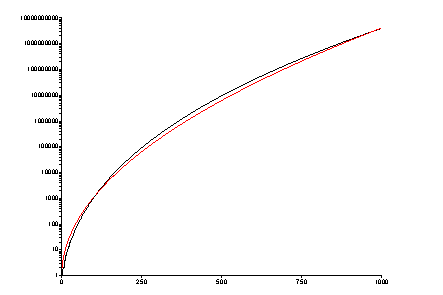
\includegraphics{squares.pdf}
\end{figure}

Figure \ref{numberReps} shows the number of such representations for $n$ up to 1000. To get a feeling
for the growth, a simple formula was guessed that approximates this number:

\begin{equation}
    F(n) \approx e^{0.7 \sqrt{n}}
\end{equation}

This formula was found by a lucky guess only and while it is fairly close to the actual number, it is
very probable that it will not work for much larger values of $n$. What is surprising, however, is that
the function $F(n)$ increases so fast.
\end{document}

